\chapter{Задание}

\section{Условие}
Структурировать исходный код программы в листинге 4.7 из исходного условия к данной лабораторной работе. Изменить программу так, чтобы она выводила на экран дерево каталогов.

Изменить функцию myftw так, чтобы каждый раз, когда встречается каталог, функции lstat() передавался не полный путь к файлу, а только его имя. Для этого после обработки всех файлов в каталоге вызовите chdir(“..”).

\section{Реализация}

\begin{lstlisting}[caption={Функция main}]
#include <stdio.h>
#include <string.h>

#include "myftw.h"

int main(int argc, char **argv)
{
    int ret;

    if (argc != 2)
    {
        fprintf(stderr, "Usage:\n    %s <input directory>\n", argv[0]);
        return 1;
    }

    ret = myftw(argv[1], myfunc);

    ntot = nreg + ndir +  nblk + nchr +  nfifo + nslink + nsock;
    if (ntot == 0)
        ntot = 1;

    char hrule[256];
    memset(hrule, '-', sizeof(hrule));

    printf("%.*s\n", 35, hrule);
    printf("Regular files: %7ld, %5.2f%%\n", nreg,   nreg   * 100.0/ntot);
    printf("Directories:   %7ld, %5.2f%%\n", ndir,   ndir   * 100.0/ntot);
    printf("Block devices: %7ld, %5.2f%%\n", nblk,   nblk   * 100.0/ntot);
    printf("Char devices:  %7ld, %5.2f%%\n", nchr,   nchr   * 100.0/ntot);
    printf("FIFOs:         %7ld, %5.2f%%\n", nfifo,  nfifo  * 100.0/ntot);
    printf("Symlinks:      %7ld, %5.2f%%\n", nslink, nslink * 100.0/ntot);
    printf("Sockets:       %7ld, %5.2f%%\n", nsock,  nsock  * 100.0/ntot);
    printf("Total:         %7ld\n",          ntot);

    return ret;
}
\end{lstlisting}
\begin{lstlisting}[caption={Объявление функции myftw, определение функции вывода, константы}]
#ifndef OSLAB02_MYFTW_H_
#define OSLAB02_MYFTW_H_

#include <stdio.h>
#include <string.h>
#include <sys/stat.h>

#define FTW_F   1 // файл, не являющийся каталогом
#define FTW_D   2 // каталог
#define FTW_DNR 3 // каталог, который не доступен для чтения
#define FTW_NS  4 // файл, о котором нельзя получить информацию

extern long nreg, ndir, nblk, nchr, nfifo, nslink, nsock, ntot;

typedef int MyFunc(const char *, const struct stat *, int, int);

static int myfunc(const char *pathname,
                  const struct stat *statptr,
                  int type, int len)
{
    for (int i = 0; i < len; i++)
            printf(" |   ");
    if (len >= 0) printf(" |--- ");

    switch (type)
    {
        case FTW_F:
            printf("%s \n", pathname);

            switch (statptr->st_mode & S_IFMT)
            {
                case S_IFREG:
                    ++nreg;
                    break;

                case S_IFBLK:
                    ++nblk;
                    break;

                case S_IFCHR:
                    ++nchr;
                    break;

                case S_IFIFO:
                    ++nfifo;
                    break;

                case S_IFLNK:
                    ++nslink;
                    break;

                case S_IFSOCK:
                    ++nsock;
                    break;

                case S_IFDIR:
                    perror("The directory is of type FTW_F");
                    return -1;
            }

            break;

        case FTW_D:
            if (pathname[strlen(pathname) - 1] == '/')
                printf("%s\n", pathname);
            else
                printf("%s/\n", pathname);
            ++ndir;
            break;

        case FTW_DNR:
            perror("Blocked access to one of the directories");
            return -1;

        case FTW_NS:
            perror("Function error stat");
            return -1;

        default:
            perror("Unknown file type");
            return -1;
    }

    return 0;
}

int myftw(char *pathname, MyFunc *func);

#endif // OSLAB02_MYFTW_H_
\end{lstlisting}
\begin{lstlisting}[caption={Рекурсивная реализация myftw}]
#include "myftw.h"

#include <sys/types.h>
#include <sys/stat.h>
#include <dirent.h>
#include <unistd.h>
#include <string.h>
#include <stdio.h>
#include <errno.h>

int dopath(MyFunc *func, char *filename, int len);

int myftw(char *pathname, MyFunc *func)
{
    return dopath(func, pathname, 0);
}

int dopath(MyFunc *func, char *filename, int len)
{
    struct stat     statbuf;
    struct dirent   *dirp;
    DIR             *dp;
    int             ret;

    if (lstat(filename, &statbuf) < 0)
        return func(filename, &statbuf, FTW_NS, len);

    if (S_ISDIR(statbuf.st_mode) == 0)
        return func(filename, &statbuf, FTW_F, len);

    ret = func(filename, &statbuf, FTW_D, len);

    if (ret != 0)
        return ret;

    dp = opendir(filename);
    if (dp == NULL)
    {
        printf("DEBUG2");
        return func(filename, &statbuf, FTW_DNR, len);
    }

    if (chdir(filename) < 0)
    {
        printf("Cannot chdir into %s\n", filename);
        return func(filename, &statbuf, FTW_DNR, len);
    }

    ++len;

    while ((dirp = readdir(dp)) != NULL)
    {
        if (strcmp(dirp->d_name, ".") != 0 &&
            strcmp(dirp->d_name, "..") != 0)
            dopath(func, dirp->d_name, len);
    }

    if (chdir("..") < 0)
    {
        printf("Cannot return into .. from %s", filename);
        return -1;
    }

    if (closedir(dp) < 0)
    {
        printf("Can't close directory %s\n", filename);
        return -1;
    }

    return ret;
}
\end{lstlisting}
\begin{lstlisting}[caption={Нерекурсивная реализация myftw}]
#include "myftw.h"

#include <sys/types.h>
#include <sys/stat.h>
#include <dirent.h>
#include <unistd.h>
#include <string.h>
#include <stdio.h>
#include <errno.h>

#include "stack.h"

int dopath(MyFunc *func, char *filename);

int myftw(char *pathname, MyFunc *func)
{
    return dopath(func, pathname);
}

int dopath(MyFunc *func, char *filename)
{
    struct stat     statbuf;
    struct dirent   *dirp;
    DIR             *dp;
    int             len = 0;

    struct stack *stack = stack_create();
    stack_push(stack, filename);

    while (!stack_is_empty(stack))
    {
        const char *filename = stack_pop(stack);

        if (strcmp(filename, "..") == 0)
        {
            --len;

            if (chdir(filename) < 0)
            {
                printf("Cannot return into .. from");
                return -1;
            }
        }
        else if (lstat(filename, &statbuf) < 0)
            func(filename, &statbuf, FTW_NS, len);
        else if (S_ISDIR(statbuf.st_mode) == 0)
            func(filename, &statbuf, FTW_F, len);
        else
        {
            func(filename, &statbuf, FTW_D, len);

            dp = opendir(filename);

            if (dp == NULL)
                func(filename, &statbuf, FTW_DNR, len);

            if (chdir(filename) < 0)
            {
                printf("Cannot chdir to %s\n", filename);
                func(filename, &statbuf, FTW_DNR, len);
            }
            else
            {
                ++len;

                stack_push(stack, "..");

                while ((dirp = readdir(dp)) != NULL)
                {
                    if (strcmp(dirp->d_name, ".")  != 0 &&
                        strcmp(dirp->d_name, "..") != 0)
                        stack_push(stack, dirp->d_name);
                }
            }
        }
    }

    return 0;
}
\end{lstlisting}
\begin{lstlisting}[caption={Объявление структуры стека и функций взаимодействия с ним}]
#ifndef OSLAB02_STACK_H_
#define OSLAB02_STACK_H_

#define STACKLIM 256

struct stack;

struct stack *stack_create();
void stack_free(struct stack **stack);

int stack_is_empty(struct stack *stack);

int stack_push(struct stack *stack, char *item);
const char *stack_pop(struct stack *stack);

#endif // OSLAB02_STACK_H_
\end{lstlisting}
\begin{lstlisting}[caption={Определение структуры стека и функций взаимодействия с ним}]
#include "stack.h"

#include <stdlib.h>

struct stack
{
    char *data[STACKLIM];
    int size;
};

struct stack *stack_create()
{
    struct stack *stack = malloc(sizeof(struct stack));
    stack->size = 0;

    return stack;
}

int stack_is_empty(struct stack *stack)
{
    return (stack->size == 0);
}

int stack_push(struct stack *stack, char *element)
{
    if (stack->size >= STACKLIM)
        return -1;

    stack->data[stack->size++] = element;

    return 0;
}

const char *stack_pop(struct stack *stack)
{
    return stack->data[--stack->size];
}

void stack_free(struct stack **stack)
{
    if (stack != NULL && *stack != NULL)
        free(*stack);

    *stack = NULL;
}
\end{lstlisting}

\section{Результаты работы}

\begin{figure}[H]
    \centering
    \caption{Сборка рекурсивной реализации и демонстрация запуска программы с неверными аргументами командной строки}
    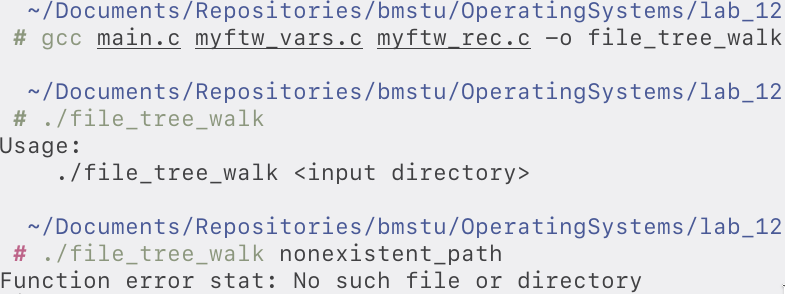
\includegraphics[scale=0.45]{images/scr_01.png}
\end{figure}
\begin{figure}[H]
    \centering
    \caption{Демонстрация работы рекурсивной реализации на примере каталога /dev, часть 1}
    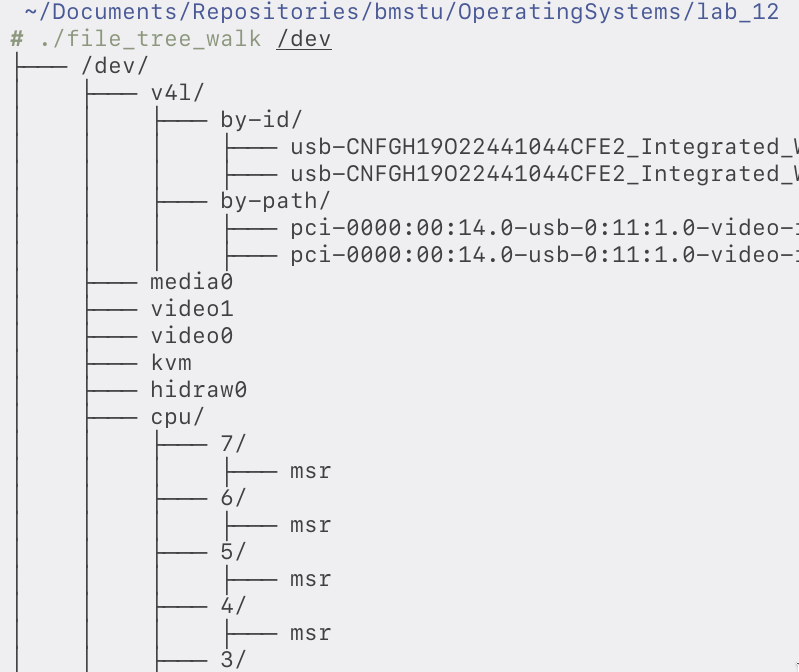
\includegraphics[scale=0.45]{images/scr_02.png}
\end{figure}
\begin{figure}[H]
    \centering
    \caption{Демонстрация работы рекурсивной реализации на примере каталога /dev, часть 2}
    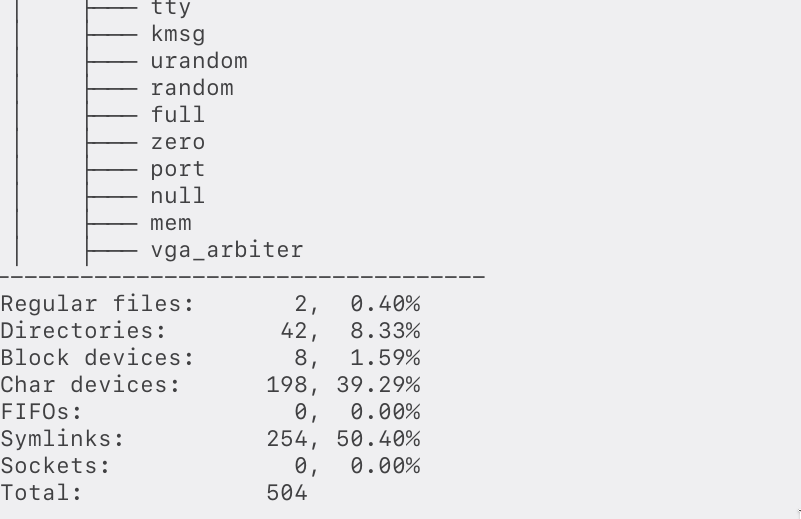
\includegraphics[scale=1.85]{images/scr_03.png}
\end{figure}
\begin{figure}[H]
    \centering
    \caption{Сборка нерекурсивной реализации и её демонстрация на примере каталога /dev, часть 1}
    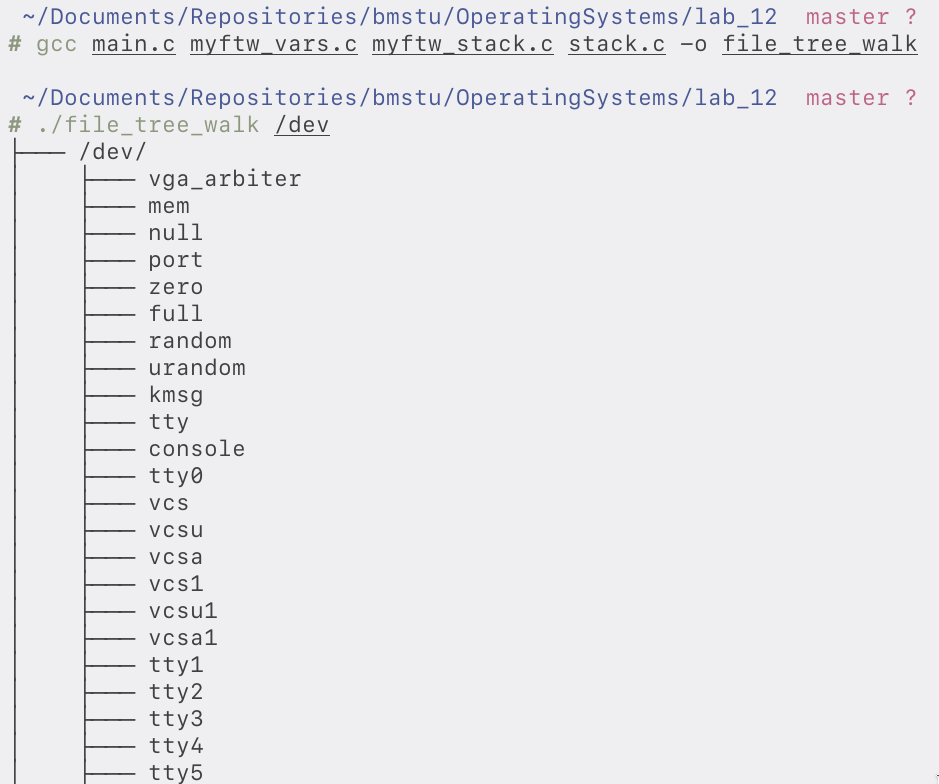
\includegraphics[scale=0.45]{images/scr_05.png}
\end{figure}
\begin{figure}[H]
    \centering
    \caption{Демонстрация работы нерекурсивной реализации на примере каталога /dev, часть 2}
    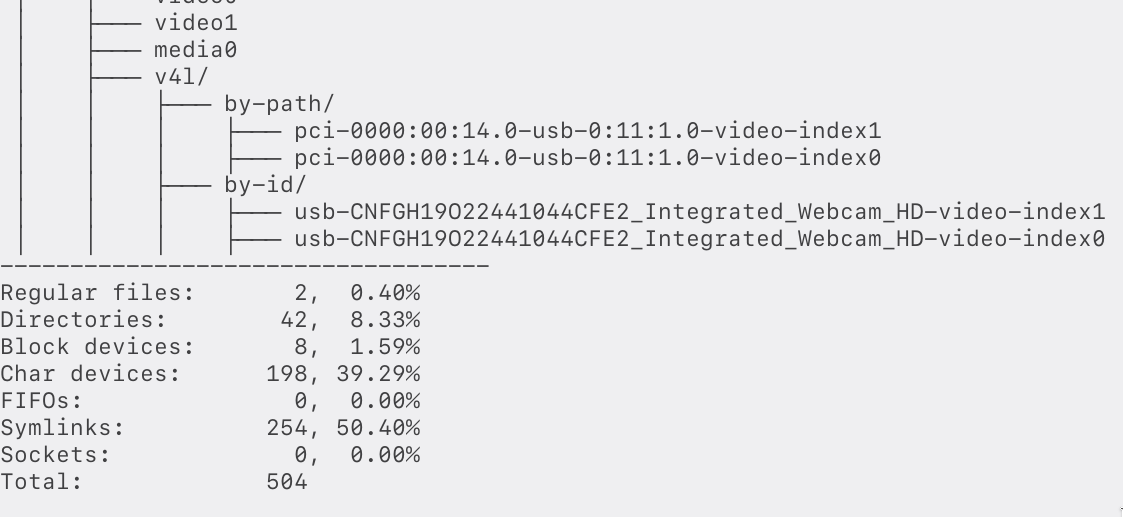
\includegraphics[scale=0.375]{images/scr_06.png}
\end{figure}

\section{Комментарии к программе}
\begin{itemize}
    \item chdir(const char *path)~--- функция смены рабочего каталога. Она устанавливает рабочий каталог, указанный в аргументе path.
    \item opendir(const char *name)~--- функция, которая открывает директорию с именем name для чтения и возвращает указатель на структуру типа DIR.
    \item closedir(DIR *dirp)~--- функция, которая закрывает поток каталога, на который указывает dirp.
    \item После обработки всех файлов в каталоге вызывается функция chdir(".."), чтобы использовать короткие имена.
    \item Функция stat заполняет структуру struct stat информацией о определённом файле. Если необходимо обнаружить символьные ссылки, следует использовать функцию lstat.
    \item lstat(const char *filename, struct stat *buf) возвращает информацию о файле с именем filename и заполняет буфер buf.
    \item S\_ISDIR~--- макрос для поля st\_mode, определяющий, является ли тип файла каталогом.
\end{itemize}
